\section{Large fields obstruct a global kernel certificate}\label{cl:sec:kernel}

Gauge integration alone does not give a uniform pointwise contraction
estimate at weak coupling. The following calculation uses the complete
$\SU(2)$ Wilson transfer kernel and an explicit admissible large field.
It concerns a global kernel certificate, not the existence of a mass gap.

Let the spatial torus have even side $L\ge6$, and put $V=L^3$.
For spatial link configurations $Q,Q'$ write
\begin{align}
A_b(Q,Q')&=\int\exp\left\{\frac b2\sum_{x,i}
\ReTr\bigl(Q_{x,i}U_{x+e_i}Q_{x,i}'{}^*U_x^*\bigr)\right\}
\prod_xdU_x,\label{cl:eq:kernel-A}\\
\mathbb T_b(Q,Q')&=D_b(Q)A_b(Q,Q')D_b(Q'),\qquad
D_b(Q)=\exp\left\{\frac b4\sum_{p\text{ spatial}}\ReTr Q_p\right\}.
\end{align}
The measure in \eqref{cl:eq:kernel-A} is product probability Haar measure.
\subsection{An explicit gap at every finite coupling and volume}
\begin{proposition}[finite-volume Wilson gap]\label{cl:prop:finite-gap}
For every finite $b>0$ and every spatial torus with sides at least three,
the $\SU(2)$ Wilson transfer operator has a simple largest eigenvalue and
\begin{equation}\label{cl:eq:finite-gap}
r_1\le\tanh\frac{3bV}{2},\qquad
m_{\rm lat}\ge-\log\tanh\frac{3bV}{2}>0.
\end{equation}
At $b=0$ it has rank one. The estimate is valid at weak coupling on each
finite lattice, but is not uniform in physical volume or cutoff.
\end{proposition}
\begin{proof}
For fixed $Q,Q'$, each term of the temporal trace sum in
\eqref{cl:eq:kernel-A} has zero product-Haar mean: the distinct endpoint
variables are independent and the mean of the defining $\SU(2)$
representation is zero. Jensen's inequality therefore gives
$A_b(Q,Q')\ge1$. Each real trace is at most two and there are $3V$
terms, so $A_b(Q,Q')\le B=e^{3bV}$.

Let $h>0$ be the continuous unit Perron eigenfunction of $\mathbb T_b$.
The associated Markov transition has density proportional to
$A_b(Q,Q')D_b(Q')h(Q')$ in its second argument. Thus all its rows are
obtained by weighting one common finite measure by functions in $[1,B]$.
Normalize that common measure to a probability $\nu$. For two such
functions $f,g$ and an event $E$ with $p=\nu(E)$, their normalized laws
$\mu_f,\mu_g$ obey
\[
\mu_f(E)-\mu_g(E)
\le\frac{Bp}{Bp+1-p}-\frac{p}{p+B(1-p)}
=\frac{(B^2-1)p(1-p)}{B+(B-1)^2p(1-p)}
\le\frac{B-1}{B+1}.
\]
The last fraction increases with $p(1-p)\le1/4$. Interchanging $f,g$
gives the same bound for the opposite difference. Hence every pair of
rows has total-variation distance at most
$\tau=(B-1)/(B+1)$, and the Markov operator satisfies
$\operatorname{osc}(Pf)\le\tau\operatorname{osc}(f)$ for bounded real $f$.

For a nonzero excited eigenvalue $r$ of $R=\mathbb T_b/\lambda_0$,
choose a real eigenfunction $u$. It is continuous, since the integral operator maps
$L^2$ into continuous functions. Compactness gives $\min h>0$, so
$u/h$ is bounded and is an eigenfunction of $P$ with eigenvalue $r$.
It is nonconstant. Consequently $r\le\tau$, proving
\eqref{cl:eq:finite-gap} since $\tau=\tanh(3bV/2)$.
Zero eigenvalues do not affect this bound. At $b=0$ the kernel is one,
which proves the rank-one assertion.
\end{proof}

The same estimate holds for every closed subgroup $G\subset\U(N_c)$,
with $b=N_c^2\beta\ge0$ and temporal exponent
$(b/N_c)\sum_e\ReTr(Q_eU_yQ_e'^*U_x^*)$.
Indeed $P_G=\int_Gg\,dg$ is the orthogonal projection onto the invariant
vectors, and $QP_G=P_GQ=P_G$ for $Q\in G$. The product-Haar mean of
each temporal real trace is therefore
$\ReTr(Q_eP_GQ_e'^*P_G)=\operatorname{Tr}P_G\ge0$.
Jensen again gives $A_b\ge1$, and $\ReTr g\le N_c$ gives
$A_b\le e^{3bV}$. Positivity of the transfer operator is
Proposition~\ref{sc:prop:wilson}; the remaining proof is unchanged.
In particular \eqref{cl:eq:finite-gap} holds at every finite positive
coupling and finite volume for every compact simple gauge group.

For a cube of fixed physical side $L$ and cutoff $a$, the volume in
\eqref{cl:eq:finite-gap} is $V=(L/a)^3$. Thus the resulting lower-bound
expression in physical units is
\[
-a^{-1}\log\tanh\!\left(\frac{3b(a)L^3}{2a^3}\right).
\]
It tends to zero as $a\downarrow0$ whenever $b(a)$ is bounded below by a
positive constant, in particular along a weak-coupling tuning. Indeed
$-\log\tanh x=\log((1+e^{-2x})/(1-e^{-2x}))\sim2e^{-2x}$ as
$x\to\infty$. The finite-volume theorem therefore gives no positive
lower bound for the continuum mass. It also does not imply that the
actual mass tends to zero.

\subsection{An admissible large-field witness}
For a positive kernel define its cross-ratio diameter by
\[
\Gamma(K)=\sup_{x,y,u,v}\log
                   \frac{K(x,u)K(y,v)}{K(x,v)K(y,u)}.
\]

\begin{theorem}[a frustrated Wilson-kernel witness]\label{cl:thm:frustrated}
For $b\ge1/4$, the gauge-integrated Wilson kernel satisfies
\begin{equation}\label{cl:eq:diameter-lower}
\Gamma(\mathbb T_b)\ge2V\max\{0,B(b)\},\qquad
B(b)=\frac{3b}{8}-\frac32\log b-\frac32-\log\frac{432\pi}{25}.
\end{equation}
The witness is invariant under passage to gauge orbits and requires no
small-field or chart restriction.
\end{theorem}
\begin{proof}
Let $Q^0_e=I$ for every link, and for $x=(x_1,x_2,x_3)$ put
\[
z_{x,1}=1,\qquad z_{x,2}=(-1)^{x_1},\qquad
z_{x,3}=(-1)^{x_1+x_2},\qquad Q^z_{x,i}=z_{x,i}I.
\]
Evenness of $L$ makes these signs periodic. In each coordinate plane
the product of the four signs on a plaquette is $-1$; hence every
spatial plaquette of $Q^z$ equals $-I$. This configuration is not gauge
equivalent to $Q^0$. Centrality and $z_e^2=1$ give
\[
A_b(Q^0,Q^0)=A_b(Q^z,Q^z)=:A_0,\qquad
A_b(Q^0,Q^z)=A_b(Q^z,Q^0)=:A_z.
\]

Identify $\SU(2)$ with the unit quaternions, using the Euclidean chord
metric $d(g,h)^2=2-\ReTr(gh^*)$. It is bi-invariant, and $d(I,-I)=2$.
For arbitrary temporal variables let $W_{x,i}=U_xz_{x,i}U_{x+e_i}^*$.
Every plaquette of $W$ is $-I$. Its four oriented links $w_1,\ldots,w_4$
therefore satisfy
\[
2\le\sum_{j=1}^4d(I,w_j),\qquad
1\le\sum_{j=1}^4d(I,w_j)^2.
\]
The first inequality is the triangle inequality applied to their
product; the second follows by Cauchy--Schwarz. Each spatial link
belongs to four plaquettes, and there are $3V$ plaquettes. Summing yields
$\sum_ed(I,W_e)^2\ge3V/4$. The mixed temporal real-trace sum is consequently
at most $6V-3V/4=21V/4$. This holds for every temporal field, and gives
\begin{equation}\label{cl:eq:frustrated-upper}
A_z\le\exp(21bV/8).
\end{equation}

For the opposite bound, restrict every $U_x$ to the chord ball
$B_\delta=\{g:d(I,g)\le\delta\}$, $0<\delta\le1$.
Adjacent variables then have distance at most $2\delta$, so the
unfrustrated temporal trace sum is at least $6V-12\delta^2V$.
Writing $g=\cos\theta+\mathbf n\sin\theta$, Haar angle measure is
$(2/\pi)\sin^2\theta\,d\theta$. The interval $0\le\theta\le\delta$
lies in $B_\delta$, and $\sin\theta\ge\theta-\theta^3/6\ge5\theta/6$
there. Hence
\[
\operatorname{Haar}(B_\delta)\ge\frac{25\delta^3}{54\pi},\qquad
A_0\ge\left(\frac{25\delta^3}{54\pi}\right)^V
                  e^{(3b-6b\delta^2)V}.
\]
For $b\ge1/4$ choose $\delta=1/(2\sqrt b)\le1$. Division by
\eqref{cl:eq:frustrated-upper} gives $A_0/A_z\ge e^{VB(b)}$.
All factors $D_b$ cancel from a cross ratio. The choice
$(x,y,u,v)=(Q^0,Q^z,Q^0,Q^z)$ therefore gives
$\Gamma(\mathbb T_b)\ge2\log(A_0/A_z)\ge2VB(b)$.
Also $\Gamma\ge0$, proving \eqref{cl:eq:diameter-lower}.
The kernels are gauge invariant in both arguments, so the same
cross ratio is defined on the gauge quotient.
\end{proof}

\begin{figure}[htbp]
\centering
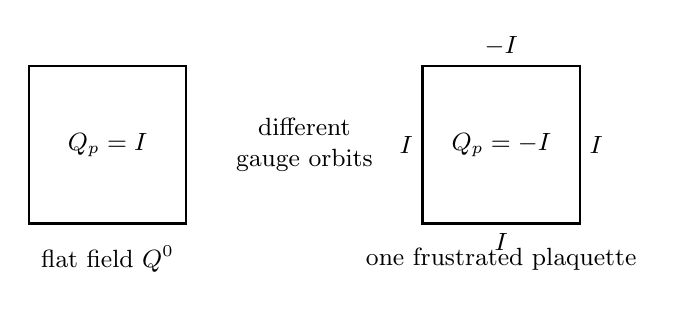
\begin{tikzpicture}[x=1cm,y=1cm,every node/.style={font=\small}]
\draw[thick] (0,0) rectangle (2,2);\node at (1,1) {$Q_p=I$};
\node at (1,-.45) {flat field $Q^0$};
\draw[thick] (5,0) rectangle (7,2);\node at (6,1) {$Q_p=-I$};
\node[above] at (6,2) {$-I$};\node[below] at (6,0) {$I$};
\node[left] at (5,1) {$I$};\node[right] at (7,1) {$I$};
\node at (6,-.45) {one frustrated plaquette};
\node[align=center] at (3.5,1) {different\\gauge orbits};
\end{tikzpicture}
\caption{A coordinate-plane plaquette of the explicit central-link
field. Every spatial plaquette is frustrated, and temporal gauge
variables cannot remove its chord-energy cost.}
\label{cl:fig:frustration}
\end{figure}

Because $B(b)\to\infty$, a certificate of the form
$\tanh(\Gamma_{\rm upper}/4)$ cannot stay below one uniformly in
coupling and volume: any valid $\Gamma_{\rm upper}$ must obey
\eqref{cl:eq:diameter-lower}.\footnote{Continuity gives the same obstruction
for an essential supremum: every neighbourhood of either witness has
positive product Haar measure. The issue is not an isolated exceptional point.}
This is not a lower bound for the actual subleading eigenvalue.
The equilibrium weight suppresses $Q^z$, and a useful averaged or
multiscale estimate could exploit that suppression. Such an estimate
must control conditional responses as well as probabilities.
For the physical cube $L=2T$, the loss in
\eqref{cl:eq:diameter-lower} is extensive in its actual volume $8T^3$.
It cannot be removed by a scalar normalisation of the transfer matrix.
